\documentclass[]{article}
\usepackage[utf8]{inputenc}
\usepackage{glossaries}
\usepackage{hyperref}
\usepackage{graphicx}


\makeglossaries

\newglossaryentry{Gamygdala}
{
	name=Gamygdala,
	description={An emotional engine created to simulate emotions for virtual identities\cite{Gamygdala}.}
}

\newglossaryentry{GOAL}
{
	name=GOAL,
	description={A programming language developed at TU Delft for creating Virtual Humans\cite{GOAL}.}
}

\newglossaryentry{virtual human}
{
	name=Virtual Human,
	description={A virtual human is an agent that uses logical rules to derive the wanted actions and can percept events from the environment. It is AI.}
}

\newglossaryentry{Tygron City Planner}
{
	name=Tygron City Planner,
	description={The serious game developed by Tygron that is played by stakeholders in urban development projects\cite{Tygron City Planner}.}
}

\newglossaryentry{Tygron}
{
	name=Tygron,
	description={The company that develops the City Planner game\cite{GOAL}.}
}


\newglossaryentry{JUnit}
{
	name=JUnit,
	description={This is a framework to build testsuites in Java.}
}

\newglossaryentry{master}
{
	name=Master,
	description={The master branch of a repository is the main of repository. Your main stable version.}
}

\newglossaryentry{packages}
{
	name=Package,
	description={a package it actually a map in which a part of your code is put. This is handy for keeping a good structure.}
}

\newglossaryentry{ANTLR}
{
	name=ANTLR,
	description={Another tool for language recognition, a framework used in GOAL to parse agent and MAS files. \cite{ANTLR}}
}

\newglossaryentry{github.com}
{
	name=github.com,
	description={A hosting website for git projects that provide convenient tools for code analysis\cite{github.com}.}
}

\newglossaryentry{CI}
{
	name=Continuous Integration,
	description={A (set of) services that continuously executes test suites and runs analyses such as test code coverage whenever changes are made\cite{CI}.}
}



% Title Page
\title{Emergent Architecture Design}
\author{GROUP: GOAL-GAMYGDALA Integration}


\begin{document}
\maketitle

\section{Introduction}
This document contains the architecture design for group 3 of the Tygron Virtual Humans project. In this document we will describe our goals during this project and how these relate to the goals of the other project groups. We will give an overview of the current architecture of GOAL as represented on the goalhub repository on github.com. Finally, we will show how the Gamygdala engine fits into the GOAL reasoning cycle, and where our other major modifications will be done.

The Tygron Virtual Humans context project aims to build a proof-of-concept system that provides the \gls{Tygron City Planner} game with virtual agents in the GOAL environment whose decisions are influenced by emotions rendered by Gamygdala. This group will develop the integration of the \gls{Gamygdala} engine in the \gls{GOAL} programming language and environment. This extended programming environment will be used by project group 1 (led by Paul Verkooijen) to write a set of agents whose decisions in the Tygron game are influenced by their emotional state. Our main purpose in this project is to provide the tools required so this group can, without having to invest time in understanding the architecture or inner workings of either GOAL or Gamygdala, use an agent's emotional state in their decisionmaking process. It is important our work renders output in the same syntax as that of the Gamygdala-plugin group led by Tom Harting so the agent group can write similar agents for both versions of GOAL-Gamygdala.
\newpage
\subsection{Goals}
As stated in the introduction, our role is a supporting one, so our goal is to support group 1 as well as possible and make working with this extended GOAL environment intuitive and similar to working with the existing GOAL language and environment that they have experience with.
Throughout the project, as our understanding of the structure of goal and the workings of gamygdala grew, we have been able to formulate clearly defined sub-goals to accomplish this task:
\begin{itemize}
  \item Integration of group 2's Gamygdala port in the GOAL package.
  \item Rendering emotions for existing GOAL agents with Gamygdala without any manual configuration or modification.
  \item Processing emotions into the belief base so that agents can reason with/about them, just like they would with percepts.
  \item Generating a default emotion configuration file that can be modified to tune the Gamygdala engine to the environment of a particular (set of) agent(s).
  \item Extending GOAL IDE so the emotional state of an agent can be read in the GOAL programming environment.
\end{itemize}

\section{Software Architecture}
This section describes various properties of the architecture of the software packages we have used or modified in this project, as well as the guidelines we have set up to ensure code quality and make use of the capabilities of the version control system we use.
\subsection{Programming languages}
Most of the development of this part of the project will be done in the Java language. The existing GOAL packages are compatible with Java 7, and therefore backwards compatible with Java 8. Gamygdala was originally written in Javascript, but we use the port to Java written by group 4. This makes development considerably easier because this port can be inserted into existing GOAL packages or referenced as a dependency in Maven projects, and we do not need to interface between Java and Javascript programs. Our modifications will be made in various packages of the GOAL architecture described in the Packages section. We need to gain some understanding of \gls{ANTLR} to be able to parse configuration for Gamygdala in GOAL at runtime. 

\subsection{Continuous Integration}
We have chosen to use git as our version control system. All project members have worked with it before and will not need much time to get reacquainted with the system. The entire GOAL project is hosted on \gls{github.com}, which is the reason we chose github for our hosting too. Cloning the existing GOAL repositories into the Tygron Virtual Humans project was a simple task compared to the work of downloading all the source code and setting it up on a different hosting service.
For continuous execution of the test suite we have chosen to use TravisCI

\subsection{Testing}
Through writing a suite of unit and integration tests we will ensure correctness of the methods and structures we add to GOAL. Since our job is to create an integration of two existing pieces of software, functionality is the most important word for our team. It should be noted that this is a proof of concept, and the time frame for this project is limited, even more so because the group that depends on our functionality will also need time to work with this GOAL version to build their agent before the end of the projec. As we focus on making sure the other groups receive the necessary features on time, some of them might be implemented quickly and dirtily. We would rather have code that ought to be rewritten sometime but works now to provide the function of a Virtual Human's gamygdala than spending a lot of time writing code that the other group cannot use because of time pressure. SCRUM seems to be the appropriate project management tool for this quick, iterative approach.
Testing of the modified software packages will be done mostly in the \gls{JUnit} framework, seeing as we are writing Java code. Because of the large pre-existing code base, its high complexity and the relatively low test coverage over these approximately 20.000 lines we have decided that achieving high coverage (>75\%, as stated in the Definition of Done in the Product Vision document) on the GOAL project is not feasible within the time frame of this project. We will focus on achieving high unit test coverage on the methods we modify, and writing integration tests that specifically target added functionality with the (faulty) assumption the pre-existing code is completely debugged, instead of spending an inordinate amount of time checking whether GOAL works as intended. Testing of the Gamygdala port was the responsibility of group 4, and they have achieved good test coverage on it. 

\subsection{Code Quality}
During this project our group will use the pull request method to develop and review code. This procedure ensures that code quality is maintained on the release branch of every github repository relevant to the project since no changes can be made without first being reviewed. This section describes the method by which we create and process these requests.
When an issue is created on github for for example new functionality, bug fixes, lack of tests or any other reason, any group member can claim the issue and open a new branch on the repository. In this personal branch modifications are made only by this group member, the changes are committed, \gls{CI} will run our test suite and the results are displayed on TravisCI and github. When the group member has finished his modification and the tests pass, he may create a pull request to merge these changes into the master branch. At least two group members other than the one making the request then review the changes and may comment on them if they have any additions or spot a mistake, prompting the requester to modify his branch accordingly. The pull request is reviewed once more, and this cycle is continued until there are no more suggestions for improvement. Then the pull request is OK'd and merged into master branch, after which the group member is free to claim another issue. This method enables the group to work more efficiently by separating several steps of the development process. Issues are created as they appear during work hours. Group members can claim issues and work on their issues on individual branches without having to communicate about who is doing what or which files in the branch are currently being modified, which means working out of the office is much less of a hassle than it would have been if we had to keep track of this by hand.
Code review is also streamlined by pull requests. For every pull request a list of changes is generated and shown on the same page, so analyzing the changes made is only a matter of a bit of scrolling. Compared to having to look through changed files manually or running git diff from the command line this is a huge improvement. With this overview and the checks ran by TravisCI, it is only a matter of a few seconds to see if a change is correct or needs some more attention.
We will attempt to keep the amount of changes in every pull request as small as possible to make reviewing them an easy task.

By using tools like Checkstyle we can maintain readability, proper line length and method size.
\newpage
\subsection{Packages}
This section gives an overview of the structure of the GOAL project, and lists the repositories in it we will modify. Here GAMYGDALA is represented as a stand-alone repository, but for convenience we have inserted it into the runtime package.\\
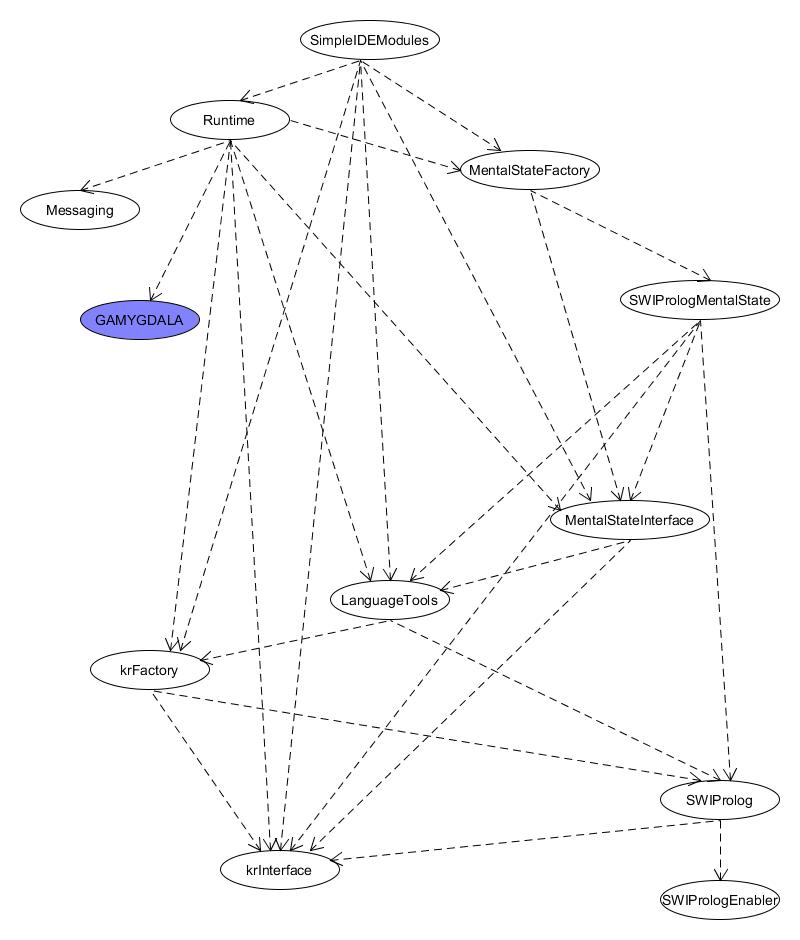
\includegraphics[scale = 0.5]{Maven_dependency_tree_UML.jpg}\\
\newpage
Throughout the project we will keep updating this list when we discover new places we need to make adjustments in.We will need to modify the following packages (or already have made adjustments):

\subsubsection{Runtime}
The packages from the runtime repository: \\ \\
\textbf{goal.core.mentalstate}: Here we extended functionality so goals that are added to agents are also added to the gamygdala engine. When goals are achieved or dropped this is also send to the Gamygdala engine. \\
\textbf{goal.core.runtime}: In this package we will need to modify the RuntimeManager. This class can be seen as the controller of GOAL. It contains the other services like the MessagingService and the EnvironmentService. This class will need to be modified to contain our Gamygdala instance. Here we will also be able to add all the agents created to the Gamygdala instance and use our emotion configuration file to add all the predefined settings to the Gamygdala instance. \\
\textbf{goal.core.runtime.service.agent}: This package is where percepts are handled and where we insert the emotions rendered by the gamygdala engine into their own EmotionBase, which is similar to the PerceptBase in the aspects that it will be flushed and repopulated every cycle and the agent should be able to reason about emotions just like reasoning about percepts. \\
\textbf{goal.tools}: The class PlatformManager resides in this package, this class has methods that retrieve the parsed version of MAS files and agent files. We modified this class to be able to parse the emotionconfig file.

\subsubsection{Grammar}
The packages from the grammar repository: \\ \\
\textbf{languageTools.parser.relationParser}: This is a subpackage we have added to the parser package to parse our emotion configuration files. It contains the parser itself and the classes needed to store the information we parsed.\\
\textbf{languageTools.exceptions.relationParser}: A package we added to contain the new exceptions thrown by our parser. \\
\textbf{languageTools.program.agent.mas}: We will need to modify the structure of the MAS file to include our emotion configuration file (in a similar way to how the MAS file contains the agent files). This specifically means adjusting the MASProgram class to contain this file. \\
\newpage
\subsubsection{MentalState}
This package needs to be modified to add the EmotionBase to the list of basetypes and will need to be extended so that prolog can do its calculations with these. GOAL has multiple bases for knowledge and beliefs and percepts (and now emotion) whereas prolog only has one knowledge base, which means all knowledge, beliefs, percepts and emotions need to be inserted into the same base before it is handed down to prolog as one knowledge base. \\

\subsubsection{SimpleIDE}
We have chosen to modify the SimpleIDE, as this would be slightly less work than modifying the Eclipse plugin, in our estimation adding GUI elements to it is fairly straightforward. We will need to add a tab like the one for percepts which displays the emotions an agent is feeling.

\clearpage
\printglossaries
\begin{thebibliography}{9}
	
	\bibitem{GOAL}
	GOAL programming language
	\url{http://ii.tudelft.nl/trac/goal}
	
	\bibitem{Gamygdala}
	Gamygdala emotion engine
	\url{http://ii.tudelft.nl/~joostb/gamygdala/index.html}
	
	\bibitem{ANTLR}
	ANTLR, another tool for language recognition
	\url{http://www.antlr.org}

	\bibitem{github.com}
	github, the online git hosting service
	\url{http://www.github.com}
	
	
\end{thebibliography}

\end{document}          
